\documentclass[onecolumn]{article}
%\usepackage{url}
%\usepackage{algorithmic}
\usepackage[a4paper]{geometry}
\usepackage{datetime}
\usepackage[margin=2em, font=small,labelfont=it]{caption}
\usepackage{graphicx}
\usepackage{float}
\usepackage{mathpazo} % use palatino
\usepackage[scaled]{helvet} % helvetica
\usepackage{microtype}
\usepackage{amsmath}
\usepackage{subfigure}
% Letterspacing macros
\newcommand{\spacecaps}[1]{\textls[200]{\MakeUppercase{#1}}}
\newcommand{\spacesc}[1]{\textls[50]{\textsc{\MakeLowercase{#1}}}}

\title{\spacecaps{Project Report}\\ \normalsize \spacesc{CENG 3521, Data Mining} }

\author{Tayyip ÖZER\\tayyipozer@posta.mu.edu.tr}
%\date{\today\\\currenttime}
\date{\today}

\begin{document}
\maketitle

\begin{abstract}
\\In this project we are going to try to train a model and predict different types of cars' prices. We are going to use data pre-processing, neural network and clustering techniques on different issues. 
\\
\end{abstract}


\section{Introduction}
I want to start with, why i chose this topic. I want to make a mobile app which can predict car prices for people who are not being aware of their car prices. So this project is going to be my start point. I find various data sets, firstly i worked on a demo which has 13.000 tuples size. Then i found bigger data sets and, while i was working on them i tried various of hidden layer size, various of attributes, various of tuple size etc. 

\\So this project was really enjoying to work on and doing my best to finish.But it is not finished for me, i will definitely want to work on similar projects. This project has two stage, first detailed data pre-processing and neural network. Let's start. 


\section{Pre-processing}
We have data of used car in USA, its dimension size is 26 and tuple size is 458,000. We have redundant dimensions and null values in the data set. It is not well distributed over years. And some dimensions like manufacturer, transmission, condition and fuel have non-numerical values so we should handle it. Let's start with getting rid of redundant dimensions. 

\subsection{Getting Rid of Redundant Dimensions}
Our data set has dimensions like unnamed, id, url, region, region url, model, cylinders, title status, VIN, drive, size, type, paint color,image url, description, state, lat, long, posting date which we drop them from our data frame. After dropping them, now we have dimensions which are price, year, manufacturer, condition, fuel, odometer and transmission.
\\

\subsection{Dropping Tuples with Null Values} 
After dropping redundant dimensions, we should drop tuples which has null values in it.In Figure~\ref{fig:fig1} we can see sum of null tuples in dimensions. After dropping null values in Figure~\ref{fig:fig2} we can see there is no null values in our data set. So finally i reset indexes and got my data set to encode it.

\begin{figure}[H]
\centering
\subfigure[Before droppings sum of null tuples]{\centering
    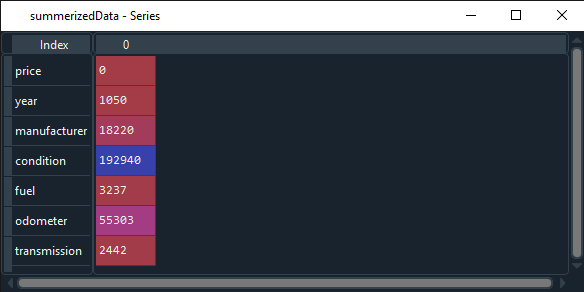
\includegraphics[width=.4\linewidth]{figures/Figure1.png}
        \label{fig:fig1}}
\subfigure[After dropping sum of null tuples]{\centering
    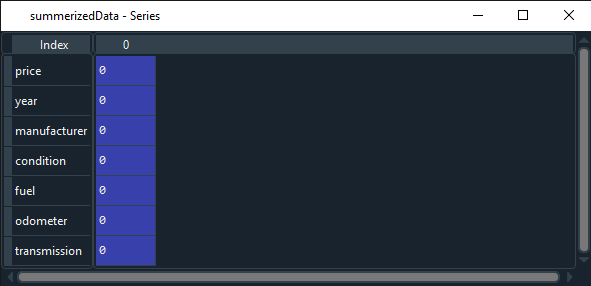
\includegraphics[width=.4\linewidth]{figures/Figure2.png}
        \label{fig:fig2}}
\caption{}
\end{figure}


\subsection{Encoding - Label - One Hot}
In our data set, as i mentioned in pre-processing, we have dimensions like manufacturer, transmission, condition and fuel which has non-numerical values in it. In Figure~\ref{fig:fig4} we can see dimensions before encoded

\begin{figure}[H]
\centering
    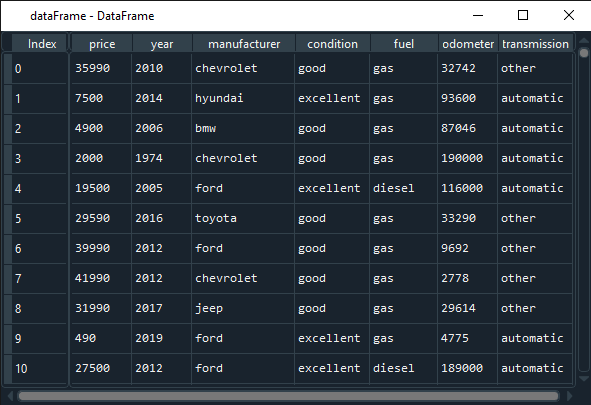
\includegraphics[width=.7\linewidth]{figures/Figure4.png}
\caption{\label{fig:fig4} Before encoding dimensions.}
\end{figure}

So we should encode them to use for model. Ways of encode them are label encoding and one-hot encoding, i used both because label encoding is not enough to order values. In Figure~\ref{fig:fig3} we can see unique labels which must be encoded.


\begin{figure}[H]
\centering
    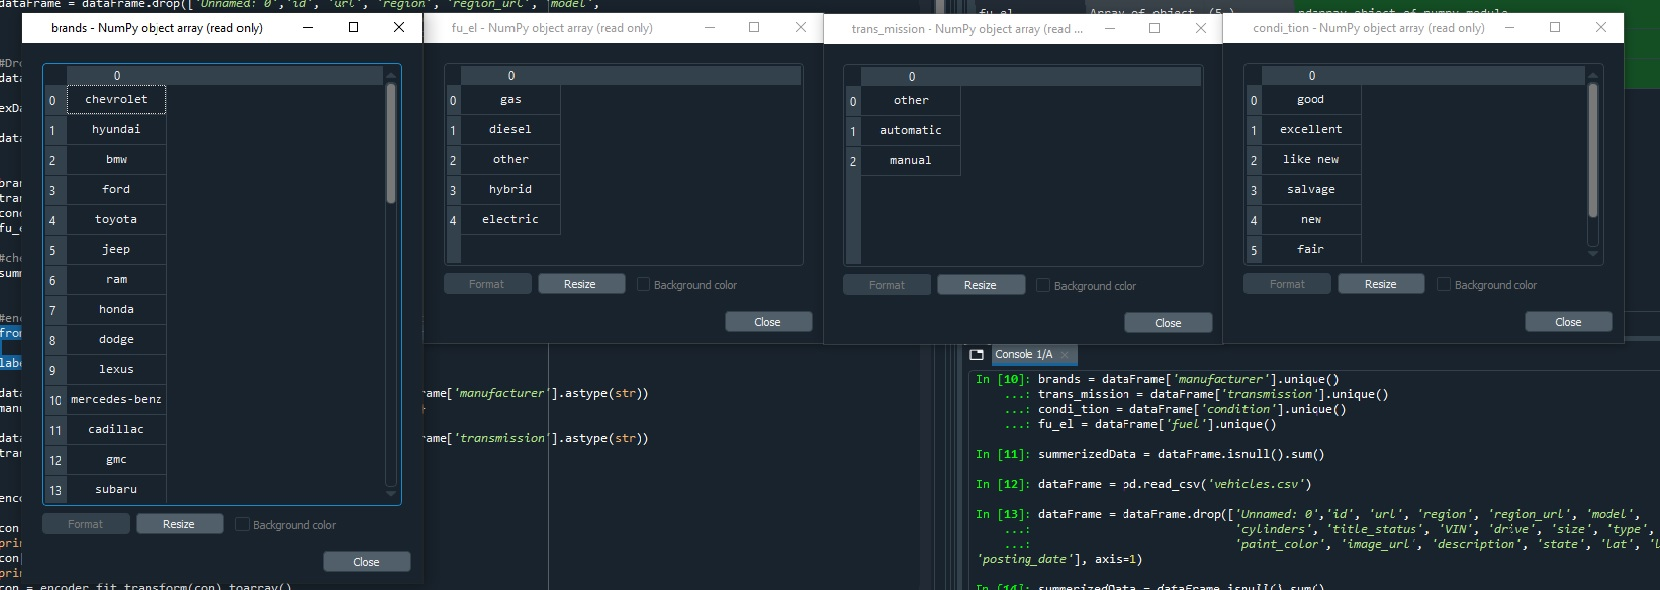
\includegraphics[width=.7\linewidth]{figures/Figure3.jpg}
\caption{\label{fig:fig3}
Unique labels which must encode.}
\end{figure}

What i mean is if you use label encoding with condition of car, label encoding gives some numbers to labels without order, it gives excellent condition to 0, fair condition to 3, good condition to 5 etc. So it is not a good way to classify them. But label encoding works with manufacturer because we cant directly say ford is greater than fiat.In Figure~\ref{fig:fig5} we can see our encoded data set.

\begin{figure}[H]
\centering
    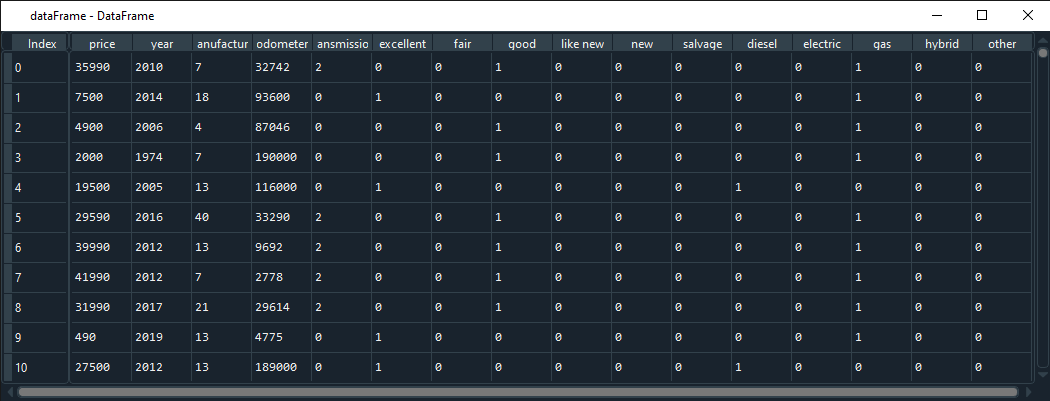
\includegraphics[width=.7\linewidth]{figures/Figure5.png}
\caption{\label{fig:fig5}
After encoding dimensions.}
\end{figure}

\subsection{Analysing and Describing Data}
With the help of the Figure~\ref{fig:fig6}, we can analyse our data and we can get some results. Let's start with talking about price, the mean price is \$31.336 which is normal, the minimum price is 0 which we should handle later because 0 prices cars are nonsense and also max prices. If we look at year, 1900's cars are not we are looking for, so we should handle minimum year. Other dimensions are looking good to continue.

\begin{figure}[H]
\centering
    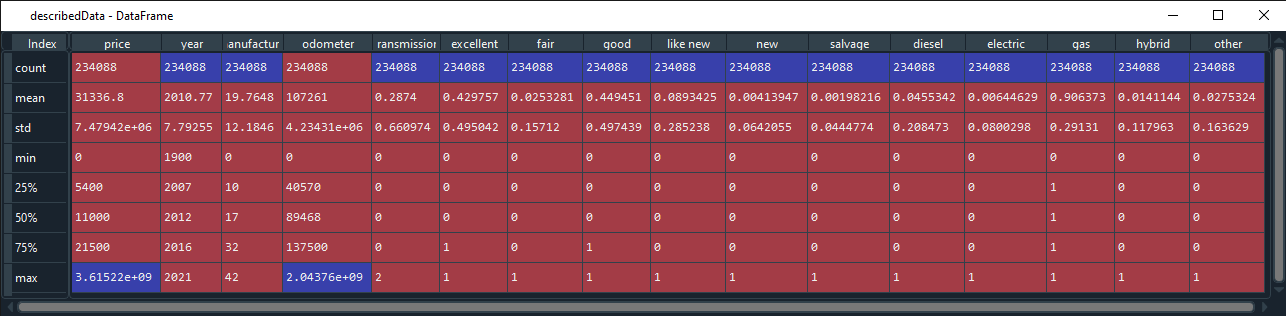
\includegraphics[width=.7\linewidth]{figures/Figure6.png}
\caption{\label{fig:fig6}
Analysing and describe of data.}
\end{figure}

\subsection{Editing and visualizing price}
Starting with Figure~\ref{fig:fig7}, as you see the distribution of price is non-sense, so we drop high prices and get a result which shown in Figure~\ref{fig:fig8}. It is better now but not enough we also drop prices lower than \$7500, getting sample with fraction 0.3 before \$20.000 and getting a result which shown in Figure~\ref{fig:fig9}. Now it is not best distributed but better.

\begin{figure}[H]
\centering
\subfigure[Before dropping really high prices]{\centering
    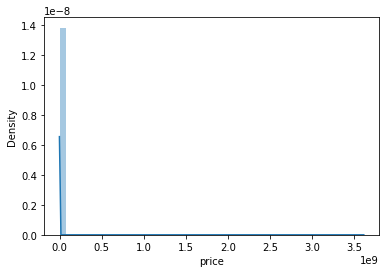
\includegraphics[width=.4\linewidth]{figures/Figure7.png}
        \label{fig:fig7}}
\subfigure[After dropping really high prices]{\centering
    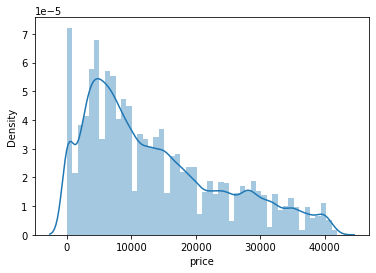
\includegraphics[width=.4\linewidth]{figures/Figure8.png}
        \label{fig:fig8}}
\subfigure[After dropping really low prices]{\centering
    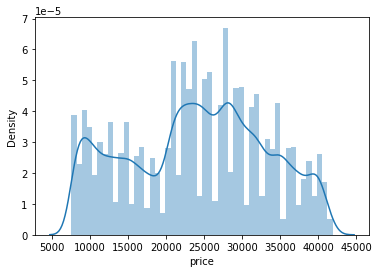
\includegraphics[width=.4\linewidth]{figures/Figure9.png}
        \label{fig:fig9}}
\caption{}
\end{figure}

\subsection{Editing and visualizing year}
Starting with Figure~\ref{fig:fig10}, as you see the distribution of year is non-sense, so we drop very early years and get a result which shown in Figure~\ref{fig:fig11}.In Figure~\ref{fig:fig12}, we can see the mean of prices grouped by years.


\begin{figure}[H]
\centering
\subfigure[Before dropping very early years]{\centering
    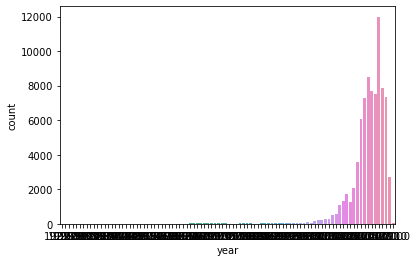
\includegraphics[width=.4\linewidth]{figures/Figure10.png}
        \label{fig:fig10}}
\subfigure[After dropping very early years]{\centering
    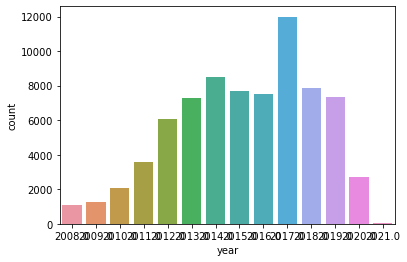
\includegraphics[width=.4\linewidth]{figures/Figure11.png}
        \label{fig:fig11}}
\subfigure[Sorted mean of prices grouped by year]{\centering
    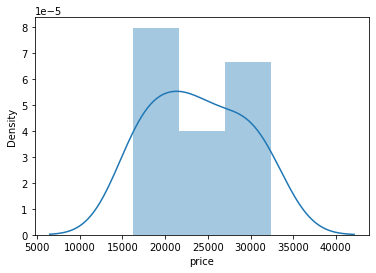
\includegraphics[width=.4\linewidth]{figures/Figure12.png}
        \label{fig:fig12}}
\caption{}
\end{figure}


\subsection{Analysing and Describing Data After Editing}
After pre-processing of our data we can see in Figure~\ref{fig:fig13}, max price and max year make sense now and other attributes also looking good.
\\
\begin{figure}[H]
\centering
       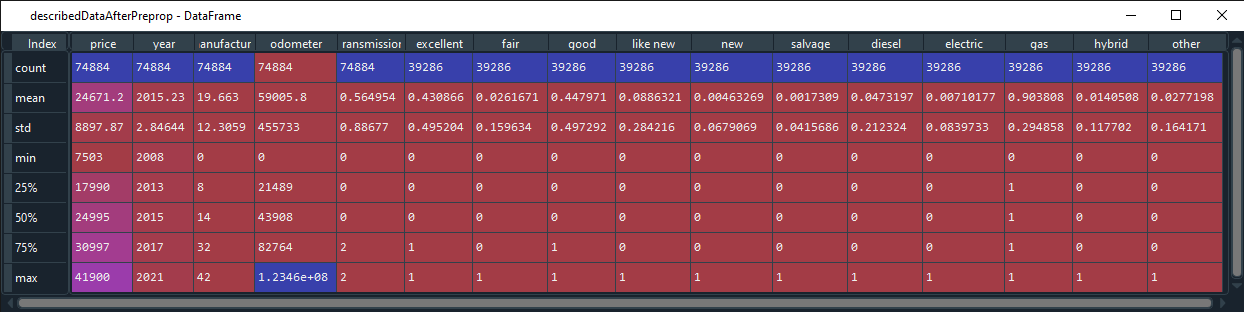
\includegraphics[width=.8\linewidth]{figures/Figure13.png}
\caption{\label{fig:fig13}
Describing data after editing.}
\end{figure}
\\
\begin{figure}[H]
\centering
    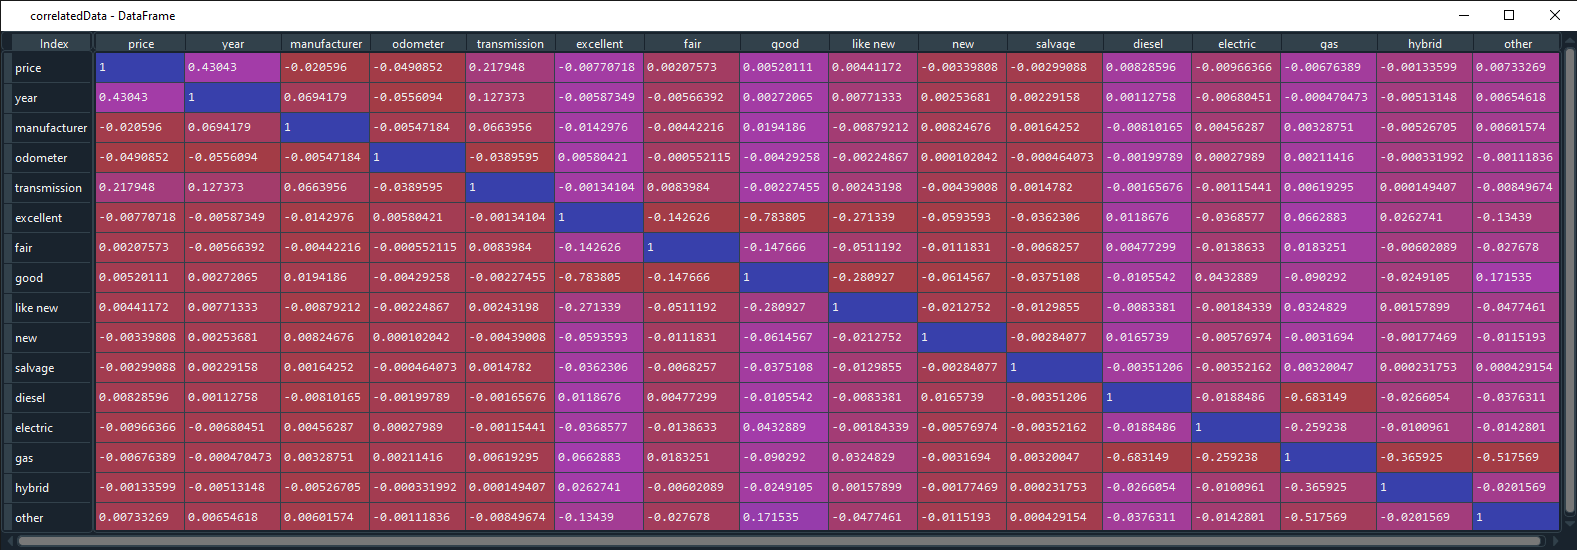
\includegraphics[width=.8\linewidth]{figures/Figure14.png}
\caption{\label{fig:fig14}
Correlated data.}
\end{figure}

In Figure~\ref{fig:fig14}, we can see correlation of all attributes each other in data set.
\begin{figure}[H]
\centering
    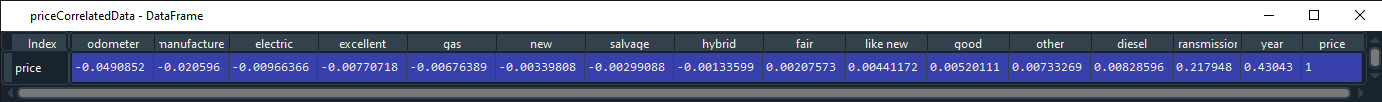
\includegraphics[width=.8\linewidth]{figures/Figure15.png}
\caption{\label{fig:fig15}
Price correlated data.}
\end{figure}
And finally in Figure~\ref{fig:fig15}, we can see correlation of price according to other dimensions. There is a some mistakes in data set, as you can see excellent condition of car has opposite relation by price. But we cant change our data set, so our data set is ready.


\section{Neural Network}
In neural network section, i used different hidden layer size and different number of neurons to find best fit. For example first i tried (64, 64, 64, 64, 64, 64), then (128, 64, 64, 32, 32, 32, 32, 16, 16, 16, 16), then (32, 32, 32, 32, 32, 32). But fitting was taking so much time so, after trying 7-8 time, i decided to leave it as this.I used mlpclassifier with 8 hidden later size each of them has 64 neurons in it. In Figure~\ref{fig:fig16}, we see loss curve of classifier.
After we train our model, we calculate mean absolute error as \$6040, that means each prediction might have approximately \$6000 error.

\begin{figure}[H]
\centering
    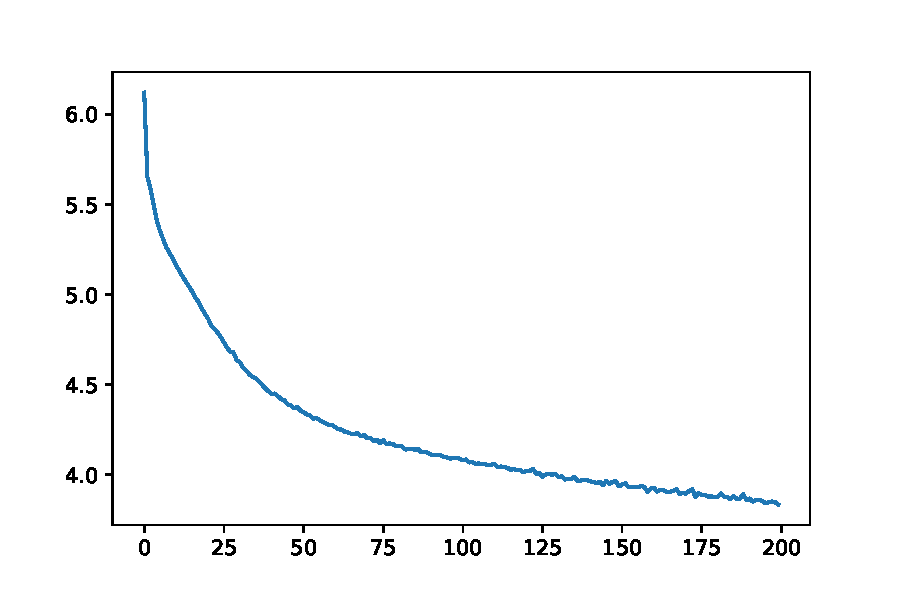
\includegraphics[width=.7\linewidth]{figures/LOSS_CURVE_.pdf}
\caption{\label{fig:fig16}
Loss curve while training model.}
\end{figure}

\section{Conclusion}
As a conclusion, we can say that, predicting car prices is a real world problem that hard to solve because of the size of research area. There are many factor which affect car prices negatively or positively. Even the total number of production of a car can affect a price of car or very old cars might be valuable. So, in my project i tried to make my research area as small as possible. I didn't use cars which have very low or high prices and i didn't use cars with very early production date. I also tried to keep the distribution of cars prices equal over the years. There were attributes which is not suitable to calculation that must be encoded. I used label and one hot encoder. Finally i train the model and find the error rate with test data. Approximately \$6000 is not really bad result for error.
It was really good experiment to have this project. I finished it with pleasure.

\nocite{*}
\bibliographystyle{plain}
\bibliography{references}
\end{document}

